
\subsection{Geometrische Anwendungen von Integralen}

\begin{Rezept}{Area($D$) - Vol($D$) - Volumen eines Normalbereichs in $\R^n$}{}
Analog zum Integrieren über Normalbereich:
\[ \text{Vol}(D) = \int_D 1 ~ dX = \underbrace{\int \!\! \int \ldots \int}_{n} 1 ~ dx_1 \ldots dx_{n-1} dx_n,  ~~~~ D \subseteq \R^n\]
\end{Rezept}

\subsubsection{Normalbereiche in $\R^2$}

\begin{Definition}{Normalbereiche in $\R^2$}{}

Sei $\Omega$ eine beschränkte Teilmenge von $\R^2$. $\Omega$ heisst \textbf{y-Normalbereich}, falls sich $\Omega$ wie folgt darstellen lässt:

\[
    \Omega = \{(x, y) \in \R^2 \mid a \leq x \leq b, f(x) \leq y \leq g(x)\}
\]

wobei $f$, $g$ stetige Funktionen der Variable $x$ sind. Die Rolle von $x$ und $y$ darf vertauscht werden (es existiert also auch ein $x$-Normalbereich).

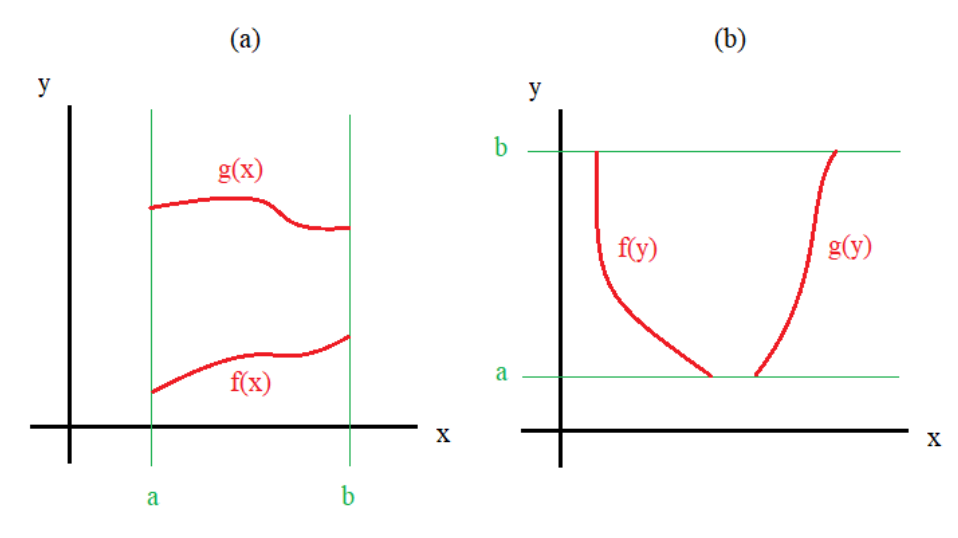
\includegraphics[width=10cm]{images/normalbereich}

(a): y-Normalbereich, (b): x-Normalbereich

\end{Definition}
\begin{Satz}{Integration auf Normalbereichen}{}

Sei \[\Omega = \{(x, y) \in \R^2 \mid a \leq x \leq b, f(x) \leq y \leq g(x)\}\] ein \textbf{y-Normalbereich} mit stetigen Funktionen $f$, $g$ und sei die zu integrierende Funktion $F \in C^0(\Omega)$, dann gilt:

\[
    \int_{\Omega} F d\mu = \int_a^b dx \int_{f(x)}^{g(x)} dy F(x, y)
\]

Das innere Integral wird zuerst ausgewertet.
\end{Satz}

\begin{Rezept}{Integrieren über Normalbereichen}{}
Am folgenden Beispiel:
\[ \int_D f(x, y) ~ dx dy ~~ \text{ wobei } ~~ D = \R^2 \cap \{(x, y) ~ | ~ y \geq 0 ~ \wedge ~ x-y+1\geq 0 ~ \wedge ~ x+2y-4 \leq 0\}\]
\begin{enumerate}
\item {
Es hilft, sich den Normalbereich visuell vorzustellen, um die Grenzen
zu finden. Bedingungen nutzen:
\[ y \geq 0 ~ \wedge (y-1 \leq x \leq 4-2y) \]
Damit $x$ nicht leer ist, muss $y-1 \leq 4-2y$ sein, resp. $y \leq \frac{5}{3}$ 
}
\item {
Für das äussere Integral sind die Integrationsgrenzen nun fest vorgegeben. Die inneren Grenzen
werden abhängig von der äusseren Variable gewählt:

\[ \int_D f(x,y) ~ dx dy = \int_0^{\frac{5}{3}} \int_{y-1}^{4-2y} f(x,y) ~ dx dy \]

}
\end{enumerate}
\end{Rezept}

\subsubsection{Satz von Green}

Dieser Satz erlaubt uns, eindimensionale Wegintegrale in zweidimensionale Gebietsintegrale umzuwandeln. D.h. wir rechnen dann jeweils die Variante aus, die einfacher geht.

\begin{Satz}{Satz von Green in der Ebene}{}
	Sei $\vec{v} = (v_1, v_2)$ ein stetig differenzierbares Vektorfeld auf einem Gebiet $\Omega \subset \R^2$ und $C \subset \R^2$ ein beschränkter Bereich mit $C^1_{pw}$ Rand $\partial C$, der sich nicht selbst schneidet. Dann gilt
	\[
		\int_{\gamma=\partial C} \vec{v} \cdot d\vec{s} = 
		\int_C \left(\frac{\partial v_2}{\partial x} - \frac{\partial v_1}{\partial y}\right) dxdy
	\]
	\textit{Bemerkung I}: Der Rand $\partial C$ muss im positiven mathematischen Sinn durchlaufen werden. D.h. das Gebiet $C$ muss jeweils links vom Rand sein, für ein Beobachter, der auf dem Rand läuft.\\
	
	\textit{Bemerkung II}: Der Satz von Green ist die zweidimensionale Version des Satzes von Stokes
\end{Satz}

\begin{Rezept}{Flächen berechnen mit Satz von Green}{}
	Gegeben: Gebiet $C \subset \R^2$ beschränkt mit $C^1_{pw}$ Rand $\partial C$.
	
	Gesucht: Fläche $F(C)$\\
	
	\textbf{Lösungsschritt I}:
	
	Parametrisiere den Rand von C mit einer Kurve
	\[
  		\gamma:[a, b] \to \R^2,\quad t \mapsto \gamma(t)
	\]
	Beachte, dass die Parametrisierung in positiver mathematischer Richtung verläuft. D.h. das Gebiet muss jeweils links der Kurve sein.
	
	\textbf{Lösungsschritt II}:
	
	Berechne $\gamma'$

	\textbf{Lösungsschritt III}:
	
	Wähle ein geeignetes Vektorfeld:
	$\frac{\partial v_2}{\partial x} -\frac{\partial v_1}{\partial y} = 1$ 
	\textbf{TODO: stimmt das wirklich für Flächenintegrale?}
	Zum Beispiel $\vec v = (0, x)$ oder $\vec v = (-y/2, x/2)$ oder $\vec v = (-y, 0)$.
	Wende dafür den Satz von Green an,
	\[
  		F(C) = \int_{\gamma=\partial C} \vec{v} \cdot d\vec{s}
	\]
\end{Rezept}

\begin{Satz}{Masse und Schwerpunkt}{}
	\textbf{TODO}	
\end{Satz}

\begin{Satz}{Satz von Stokes}{}
	\textbf{Hinweis}: Dieser Satz kam nicht in der Vorlesung vor. Er ist eine Verallgemeinerung des Satzes von Green.	
\end{Satz}

\subsubsection{Satz von Gauss}

\begin{Satz}{Satz von Gauss}{}
	\textbf{TODO}	
\end{Satz}


